\documentclass[11pt]{article}

% some definitions for the title page
\newcommand{\reporttitle}{Introduction Lecture for NLP and some ML baselines}
\newcommand{\reportdescription}{THe introductory lecture for Natural Language Processing and some core concepts for Natural Language Processing with supplementary material regarding basic ML concepts required for this course}

% load some definitions and default packages
%---------------------------------------------------------------------------
%	PACKAGES AND OTHER DOCUMENT CONFIGURATIONS
%---------------------------------------------------------------------------

\usepackage[twoside]{fancyhdr}
\usepackage{csquotes}

\usepackage[a4paper,hmargin=2.0cm,vmargin=1.0cm,includeheadfoot]{geometry}
% \usepackage{natbib} % for bibliography
\usepackage{biblatex}
\usepackage{tabularx,longtable,multirow,subfigure,caption}%hangcaption
\usepackage{fancyhdr} % page layout
\usepackage{url} % URLs
\usepackage[english]{babel}
\usepackage{graphicx}
\usepackage{rotating}
\usepackage{dsfont}
\usepackage{epstopdf} % automatically replace .eps with .pdf in graphics
% \usepackage{backref} % needed for citations
\usepackage{array}
\usepackage{latexsym}
\usepackage[pdftex,hypertexnames=false,colorlinks]{hyperref} % provide links in pdf (had pagebackref)
\usepackage{booktabs}
\usepackage{wrapfig}
\usepackage{caption}  % Required for \captionof
\usepackage{float} % for H option in figures
\usepackage{amssymb}
\usepackage{amsmath}
\usepackage{amsthm}
\usepackage{mathtools} % for 'dcases*' env.
\usepackage[nottoc]{tocbibind}

%%% Default fonts
\renewcommand*{\rmdefault}{bch}
\renewcommand*{\ttdefault}{cmtt}

%%% Default settings (page layout)
\setlength{\parindent}{0em}  % indentation of paragraph
\setlength{\parskip}{.3em}
\setlength{\itemsep}{0.mm}

\setlength{\headheight}{14.5pt}
\pagestyle{fancy}

\fancyfoot[ER,OL]{\thepage}%Page no. in the left on odd pages and on right on even pages

\fancyfoot[OC,EC]{\sffamily }
\renewcommand{\headrulewidth}{0.1pt}
\renewcommand{\footrulewidth}{0.1pt}
\captionsetup{margin=10pt,font=small,labelfont=bf}

% LISTINGS ammendments
\usepackage{listings}
\usepackage{color}

\definecolor{mygreen}{rgb}{0,0.6,0}
\definecolor{mygray}{rgb}{0.5,0.5,0.5}
\definecolor{mymauve}{rgb}{0.58,0,0.82}

\lstset{ 
  postbreak=\mbox{\textcolor{red}{$\hookrightarrow$}\space},
  backgroundcolor=\color{white},   % choose the background color; you must add \usepackage{color} or \usepackage{xcolor}; should come as last argument
  basicstyle=\footnotesize,        % the size of the fonts that are used for the code
  breakatwhitespace=false,         % sets if automatic breaks should only happen at whitespace
  breaklines=true,                 % sets automatic line breaking
  captionpos=b,                    % sets the caption-position to bottom
  commentstyle=\color{mygreen},    % comment style
%   deletekeywords={...},            % if you want to delete keywords from the given language
%   escapeinside={\%*}{*)},          % if you want to add LaTeX within your code
  extendedchars=true,              % lets you use non-ASCII characters; for 8-bits encodings only, does not work with UTF-8
  firstnumber=1,                % start line enumeration with line 1000
  frame=single,	                   % adds a frame around the code
  keepspaces=true,                 % keeps spaces in text, useful for keeping indentation of code (possibly needs columns=flexible)
  columns=fullflexible,
  keywordstyle=\color{blue},       % keyword style
  language=python,                 % the language of the code
  % morekeywords={*,...},            % if you want to add more keywords to the set
  numbers=left,                    % where to put the line-numbers; possible values are (none, left, right)
  numbersep=5pt,                   % how far the line-numbers are from the code
  numberstyle=\tiny\color{mygray}, % the style that is used for the line-numbers
  rulecolor=\color{black},         % if not set, the frame-color may be changed on line-breaks within not-black text (e.g. comments (green here))
  showspaces=false,                % show spaces everywhere adding particular underscores; it overrides 'showstringspaces'
  showstringspaces=false,          % underline spaces within strings only
  showtabs=false,                  % show tabs within strings adding particular underscores
  stepnumber=1,                    % the step between two line-numbers. If it's 1, each line will be numbered
  stringstyle=\color{mymauve},     % string literal style
  tabsize=2,	                   % sets default tabsize to 2 spaces
  title=\lstname% show the filename of files included with \lstinputlisting; also try caption instead of title
}

% Here, you can define your own macros. Some examples are given below.

\newcommand{\R}[0]{\mathds{R}} % real numbers
\newcommand{\Z}[0]{\mathds{Z}} % integers
\newcommand{\N}[0]{\mathds{N}} % natural numbers
\newcommand{\C}[0]{\mathds{C}} % complex numbers
\renewcommand{\vec}[1]{{\boldsymbol{{#1}}}} % vector
\newcommand{\mat}[1]{{\boldsymbol{{#1}}}} % matrix


\bibliography{../bibliography}

\begin{document}

% Include the title page
\begin{titlepage}

    \newcommand{\HRule}{\rule{\linewidth}{0.5mm}} % Defines a new command for the horizontal lines, change thickness here
    
    \center % Center everything on the page
     
    %------------------------------------------------------------------------
    %	HEADING SECTIONS
    %------------------------------------------------------------------------
    
    \textsc{\Large Department of Computing}\\[0.5cm] 
    \textsc{\large Imperial College of Science, Technology and Medicine}\\[0.5cm] 
    
    %------------------------------------------------------------------------
    %	TITLE SECTION
    %------------------------------------------------------------------------
    
    \HRule \\[0.4cm]
    { \huge \bfseries \reporttitle}\\ % Title of your document
    \HRule \\[0.4cm]

    \textit{\reportdescription}
    
    \vspace{2em}

    %------------------------------------------------------------------------
    %	AUTHOR SECTION
    %------------------------------------------------------------------------
    
    \large \emph{Author: Anton Zhitomirskiy}

    \vspace{1em}

    \global\let\newpagegood\newpage
    \global\let\newpage\relax
    
\end{titlepage}

\global\let\newpage\newpagegood

\tableofcontents

\clearpage

\section{Dealing with natural language}

\subsection{Complexities}

\begin{itemize}
    \item Ambiguity at word level
          \begin{quote}
            ``Can you bring me the file''
        \end{quote}
    \item Syntactic ambiguity (prepositional phrase attachment ambiguity)
          \begin{quote}
            ``I saw the boy with a telescope''
        \end{quote}
    \item Semantic ambiguity
          \begin{quote}
            ``I haven't slept for 10 days''
            ``The rabbit is ready for lunch''
        \end{quote}
    \item Referential ambiguity
          \begin{quote}
            ``We gave the monkeys bananas because they were more than ready to eat.''
        \end{quote}
    \item Non-literal meaning
          \begin{quote}
            ``Call me a cab, it's raining cats and dogs''
        \end{quote}
\end{itemize}

\subsection{The role of Deep Learning}

\begin{itemize}
    \item The creation and maintenance of linguistic rules often is infeasible or impractical.
    \item We'd much rather learn functions from data instead of creating rules based on intuition.
    \item deep learning is very flexible, learnable framework fro representing information from many different modalities.
\end{itemize}

\subsection{Composites of Language}

\subsubsection{Lexicon - morphological analysis}

Definition: Words: segmentation, normalisation, morphology

\begin{enumerate}
    \item Word Segmentation (tokenization, decompounding): 
    \begin{quote}
        ``For example, most of what we are going to do with language relies on first separating out or tokenizing words from running text, the task of tokenization. English words are often separated from each other tokenization by whitespace, but whitespace is not always sufficient. ``New York'' and ``rock 'n' roll'' are sometimes treated as large words despite the fact that they contain spaces, while sometimes we'll need to separate ``I'm'' into the two words ``I and am''''~\cite{book-speech-and-language-processing}
    \end{quote}
    \item Word normalization (capitalization, acronyms, spelling variants)
    \item Lemmatisation (reduce to base form = valid word)
    \begin{quote}
        ``Another part of text normalization is lemmatization, the task of determining lemmatization that two words have the same root, despite their surface differences. For example, the words sang, sung, and sings are forms of the verb sing. The word sing is the common lemma of these words, and a lemmatizer maps from all of these to sing''~\cite{book-speech-and-language-processing}
    \end{quote}
    \item Stemming (reduce to root = not always valid word)
    \begin{quote}
        ``Stemming refers to a simpler version of lemmatization in which we mainly stemming just strip suffixes from the end of the word''~\cite{book-speech-and-language-processing}.
    \end{quote}
    \item Byte-pair encoding (BPE) and wordpieces
    \begin{quote}
        ``Instead of defining tokens as words (whether delimited by spaces or more complex algorithms), or as characters (as in Chinese), we can use our data to automatically tell us what the tokens should be''~\cite{book-speech-and-language-processing}.
    \end{quote}

    \begin{figure}[H]
        \centering
        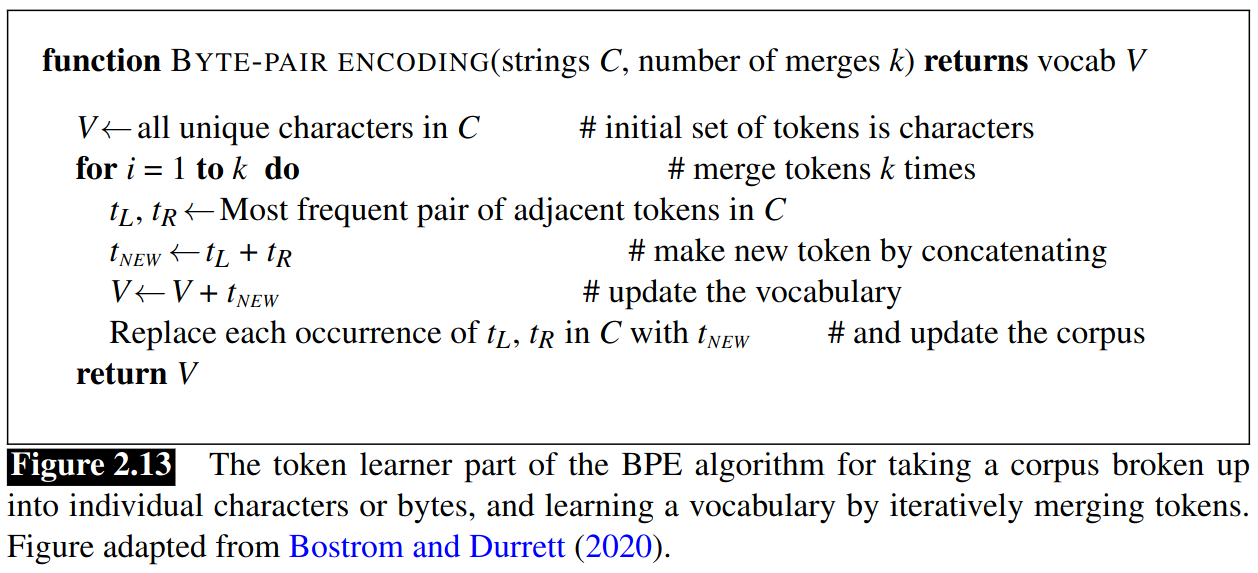
\includegraphics[width=.8\linewidth]{figures/bpe-algorithm.png}
        \label{fig:bpe-algorithm}
    \end{figure}

    \begin{quote}
        ``The BPE token learner begins BPE with a vocabulary that is just the set of all individual characters. It then examines the training corpus, chooses the two symbols that are most frequently adjacent (say 'A', 'B'), adds a new merged symbol 'AB' to the vocabulary, and replaces every adjacent 'A' 'B' in the corpus with the new 'AB'. It continues to count and merge, creating new longer and longer character strings, until k merges have been done creating k novel tokens; k is thus a parameter of the algorithm. The resulting vocabulary consists of the original set of characters plus k new symbols''~\cite{book-speech-and-language-processing}.
    \end{quote}

    \item Part-of-speech tagging (Recognize category of word): verb, noun, adverb, adjective, determiner, preposition... 
    
    It is the process of assigning a part-of-speech to each word in a text. This is a disambiguation task; words are ambiguous - have more tha one possible part-of-speech - and the goal is to find the correct tag for the sitauation. E.g. `book' can be a verb (`book that flight') or a noun (`hand me that book'). The POS-tagging resolves these ambiguities by choosing the proper tag for the context~\cite{book-speech-and-language-processing}.

    \item Morphological analysis (recognize/generate word variants):
    
    \begin{quote}
        ``Morphology is the study of the way words are built up from smaller meaning-bearing units called morphemes. Two broad classes of morphemes can be distinguished: \textbf{stems} — the central morpheme of the word, supplying the main meaning — and \textbf{affixes} — adding “additional” meanings of various kinds. So, for example, the word fox consists of one morpheme (the morpheme fox) and the word cats consists of two: the morpheme cat and the morpheme `-s'''~\cite{book-speech-and-language-processing}
    \end{quote}
\end{enumerate}

\subsubsection{Syntax}

Syntax comes from the Greek s'yntaxis, meaning “setting out together or arrangement”, and refers to the way words are arranged together~\cite{book-speech-and-language-processing}.

We can form a parse tree based on some syntax rules which makes up grammar. This was typically used in applications before deep learning; there are sentences that make sense but don't follow grammar.

\begin{tabular}{l c r}
    \hline
    \multicolumn{2}{c}{\textbf{Phrase Structure Rule}} & \textbf{Example} \\
    \hline
    $S \rightarrow NP \quad VP$ & Sentence $\rightarrow$ Noun-phrase Verb-phrase & I prefer a morning flight \\
    $NP \rightarrow Det\ N$ & Noun-phrase $\rightarrow$ Determiner Noun & prefer a morning flight\\
    $VP \rightarrow V NP$ & Verb-phrase $\rightarrow$ Verb Noun-phrase & leave Boston in the morning\\
    $VP \rightarrow V$ & Verb-phrase $\rightarrow$ Verb & \\
    $VP \rightarrow V PP$ & Verb-phrase $\rightarrow$ Verb Propositional-phrase & leaving on Thursday\\
    $PP \rightarrow P NP$ & Preposition-phrase $\rightarrow$ Preposition Noun-phrase & from Los Angeles\\
\end{tabular}

\subsubsection{Semantics}

Definition: Meaning of words and sentences

``We also introduce word sense disambiguation (WSD), the task of determining which sense of a word is being used in a particular context [...] A sense (or word sense) is a discrete representation of one aspect of the meaning of a word.''~\cite{book-speech-and-language-processing}.

Compositional meaning understands who did what to whom, when, where, how and why. It composes the meaning of the setnece, based on the meaning of the words and the structure of the sentence. Here, the dog chased the man = The man was chased by the dog, but The dog bit the man $\neq$ The man bit the dog.

``Semantic role labeling (sometimes shortened as SRL) is the task of automatically finding the semantic roles of each argument of each predicate in a sentence''~\cite{book-speech-and-language-processing}.

\subsubsection{Discourse}

Definition: Meaning of a text (relationship between sentences)

``language does not normally consist of isolated, unrelated sentences, but instead of collocated, structured, coherent groups of sentences. We refer to such a coherent structured group of sentences as a discourse, and we use the word coherence to refer to the relationship between sentences that makes real discourses different than just random assemblages of sentences''~\cite{book-speech-and-language-processing}.

``Coreference resolution is the task of determining whether two mentions corefer, by which we mean they refer to the same entity in the discourse model (the same discourse entity)''~\cite{book-speech-and-language-processing}.

\subsubsection{Pragmatics}

Definition: Intentions, commands; what is the intent of the text, how to react to it?

\section{Word Representation}

\subsection{One-hot-encoding}

\begin{itemize}
    \item Corpus: A collection of documents, i.e. our entire dataset
    \item Document: one item of our corpus (e.g. a sequence)
    \item token: the atomic unit of a sequence (e.g. a word)
    \item vocabulary: the unique tokens across our entire corpus
\end{itemize}

\end{document}